\section{Results}
\label{sec:results}
In this section, we will present the results of EVOLVE framework. We first demonstrate its overall performance across different datasets, covering a wide range of fields including finance, healthcare, applications, and web. Next, we demonstrate EVOLVE's effective evolution on python guardrail tools. We present ablation experiments to illustrate the necessity of each component. We also conduct a case study in the AI2THOR simulation environment to demonstrate the real-world significance of EVOLVE framework. Cases of generated guardrail tools are in Appendix~\ref{appendix:toolcase} and cases of tool evolution are in Appendix~\ref{appendix:toolevolutioncase}.

\subsection{Benchmark Performance Evaluation}
% \begin{figure}
%     \centering
%     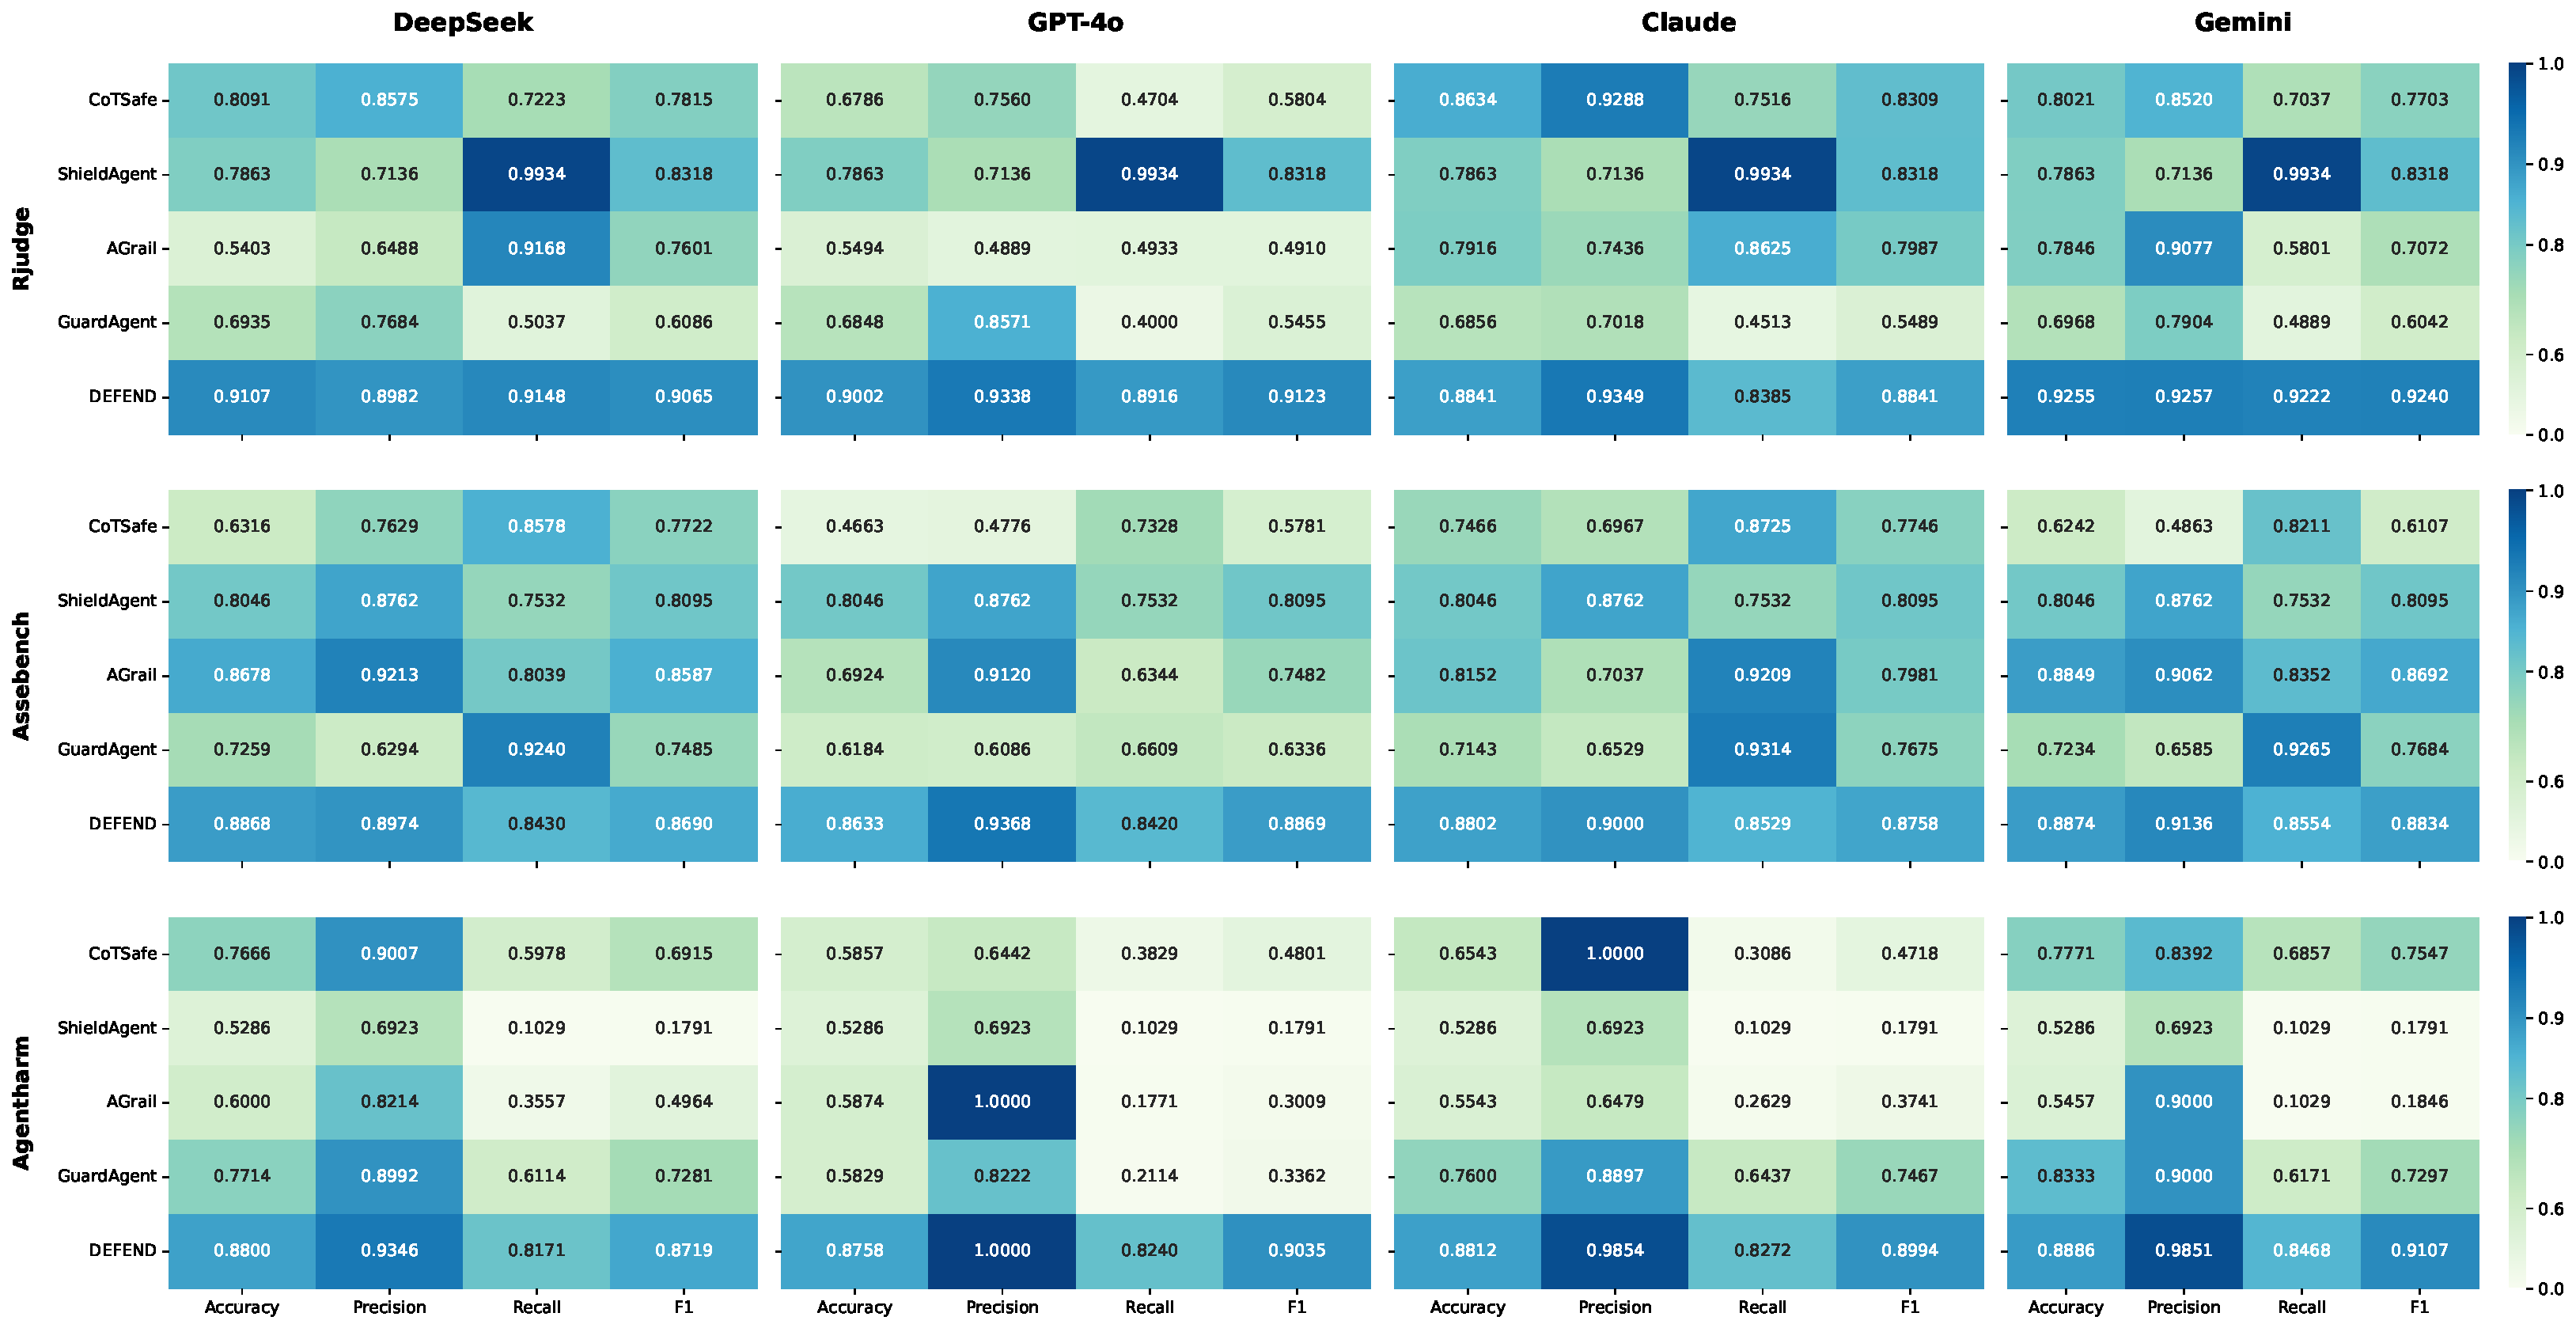
\includegraphics[width=\linewidth]{code/main_result.pdf}
%     \caption{Main results of the five frameworks on three benchmarks. Heatmap shows the performance of each framework across different metrics, with darker colors indicating better performance. EVOLVE performs well, significantly outperforming the baseline across multiple metrics.}
%     \label{fig:main_result}
% \end{figure}
% \begin{table*}[ht]
\centering
\caption{Results across three benchmarks and four backbone LLMs.
\textbf{Bold} indicates the best, \underline{Underline} indicates the second.
\textsuperscript{$\dagger$}ShieldAgent does not rely on a backbone LLM, its scores are identical across all groups.}
\label{tab:main_results}
\renewcommand{\arraystretch}{1.2}
\setlength{\tabcolsep}{4.5pt}
\resizebox{\textwidth}{!}{%
\begin{tabular}{lcccccccccccc}
\toprule
&
\multicolumn{4}{c}{\textbf{RJudge}} &
\multicolumn{4}{c}{\textbf{AsseBench}} &
\multicolumn{4}{c}{\textbf{AgentHarm}} \\
\cmidrule(lr){2-5}\cmidrule(lr){6-9}\cmidrule(lr){10-13}
\textbf{Method} &
Acc & Prec & Rec & F1 &
Acc & Prec & Rec & F1 &
Acc & Prec & Rec & F1 \\
\midrule

% ── DeepSeek ──────────────────────────────────────────────────
\multicolumn{13}{c}{\textit{Backbone LLM: DeepSeek}} \\[2pt]
CoTSafe
  & \underline{0.8091} & \underline{0.8575} & 0.7223 & 0.7815
  & 0.6316 & 0.7629 & \underline{0.8578} & 0.7722
  & 0.7666 & \underline{0.9007} & 0.5978 & 0.6915 \\
ShieldAgent\textsuperscript{$\dagger$}
  & 0.7863 & 0.7136 & \textbf{0.9934} & \underline{0.8318}
  & 0.8046 & 0.8762 & 0.7532 & 0.8095
  & 0.5286 & 0.6923 & 0.1029 & 0.1791 \\
AGrail
  & 0.5403 & 0.6488 & \underline{0.9168} & 0.7601
  & \underline{0.8678} & \textbf{0.9213} & 0.8039 & \underline{0.8587}
  & 0.6000 & 0.8214 & 0.3557 & 0.4964 \\
GuardAgent
  & 0.6935 & 0.7684 & 0.5037 & 0.6086
  & 0.7259 & 0.6294 & \textbf{0.9240} & 0.7485
  & \underline{0.7714} & 0.8992 & \underline{0.6114} & \underline{0.7281} \\
\textbf{EVOLVE}
  & \textbf{0.9107} & \textbf{0.8982} & 0.9148 & \textbf{0.9065}
  & \textbf{0.8868} & \underline{0.8974} & 0.8430 & \textbf{0.8690}
  & \textbf{0.8800} & \textbf{0.9346} & \textbf{0.8171} & \textbf{0.8719} \\

\midrule

% ── GPT-4o ────────────────────────────────────────────────────
\multicolumn{13}{c}{\textit{Backbone LLM: GPT-4o}} \\[2pt]
CoTSafe
  & 0.6786 & 0.7560 & 0.4704 & 0.5804
  & 0.4663 & 0.4776 & 0.7328 & 0.5781
  & 0.5857 & 0.6442 & \underline{0.3829} & \underline{0.4801} \\
ShieldAgent\textsuperscript{$\dagger$}
  & \underline{0.7863} & 0.7136 & \textbf{0.9934} & \underline{0.8318}
  & \underline{0.8046} & 0.8762 & \underline{0.7532} & \underline{0.8095}
  & 0.5286 & 0.6923 & 0.1029 & 0.1791 \\
AGrail
  & 0.5494 & 0.4889 & 0.4933 & 0.4910
  & 0.6924 & \underline{0.9120} & 0.6344 & 0.7482
  & \underline{0.5874} & \textbf{1.0000} & 0.1771 & 0.3009 \\
GuardAgent
  & 0.6848 & \underline{0.8571} & 0.4000 & 0.5455
  & 0.6184 & 0.6086 & 0.6609 & 0.6336
  & 0.5829 & \underline{0.8222} & 0.2114 & 0.3362 \\
\textbf{EVOLVE}
  & \textbf{0.9002} & \textbf{0.9338} & \underline{0.8916} & \textbf{0.9123}
  & \textbf{0.8633} & \textbf{0.9368} & \textbf{0.8420} & \textbf{0.8869}
  & \textbf{0.8758} & \textbf{1.0000} & \textbf{0.8240} & \textbf{0.9035} \\

\midrule

% ── Claude ────────────────────────────────────────────────────
\multicolumn{13}{c}{\textit{Backbone LLM: Claude}} \\[2pt]
CoTSafe
  & \underline{0.8634} & \underline{0.9288} & 0.7516 & 0.8309
  & 0.7466 & 0.6967 & 0.8725 & 0.7746
  & 0.6543 & \textbf{1.0000} & 0.3086 & 0.4718 \\
ShieldAgent\textsuperscript{$\dagger$}
  & 0.7863 & 0.7136 & \textbf{0.9934} & \underline{0.8318}
  & 0.8046 & \underline{0.8762} & 0.7532 & \underline{0.8095}
  & 0.5286 & 0.6923 & 0.1029 & 0.1791 \\
AGrail
  & 0.7916 & 0.7436 & \underline{0.8625} & 0.7987
  & \underline{0.8152} & 0.7037 & \underline{0.9209} & 0.7981
  & 0.5543 & 0.6479 & 0.2629 & 0.3741 \\
GuardAgent
  & 0.6856 & 0.7018 & 0.4513 & 0.5489
  & 0.7143 & 0.6529 & \textbf{0.9314} & 0.7675
  & \underline{0.7600} & 0.8897 & \underline{0.6437} & \underline{0.7467} \\
\textbf{EVOLVE}
  & \textbf{0.8841} & \textbf{0.9349} & 0.8385 & \textbf{0.8841}
  & \textbf{0.8802} & \textbf{0.9000} & 0.8529 & \textbf{0.8758}
  & \textbf{0.8812} & \underline{0.9854} & \textbf{0.8272} & \textbf{0.8994} \\

\midrule

% ── Gemini ────────────────────────────────────────────────────
\multicolumn{13}{c}{\textit{Backbone LLM: Gemini}} \\[2pt]
CoTSafe
  & \underline{0.8021} & 0.8520 & 0.7037 & 0.7703
  & 0.6242 & 0.4863 & 0.8211 & 0.6107
  & 0.7771 & 0.8392 & \underline{0.6857} & \underline{0.7547} \\
ShieldAgent\textsuperscript{$\dagger$}
  & 0.7863 & 0.7136 & \textbf{0.9934} & \underline{0.8318}
  & 0.8046 & 0.8762 & 0.7532 & 0.8095
  & 0.5286 & 0.6923 & 0.1029 & 0.1791 \\
AGrail
  & 0.7846 & \underline{0.9077} & 0.5801 & 0.7072
  & \underline{0.8849} & \underline{0.9062} & 0.8352 & \underline{0.8692}
  & 0.5457 & \underline{0.9000} & 0.1029 & 0.1846 \\
GuardAgent
  & 0.6968 & 0.7904 & 0.4889 & 0.6042
  & 0.7234 & 0.6585 & \textbf{0.9265} & 0.7684
  & \underline{0.8333} & \underline{0.9000} & 0.6171 & 0.7297 \\
\textbf{EVOLVE}
  & \textbf{0.9255} & \textbf{0.9257} & \underline{0.9222} & \textbf{0.9240}
  & \textbf{0.8874} & \textbf{0.9136} & \underline{0.8554} & \textbf{0.8834}
  & \textbf{0.8886} & \textbf{0.9851} & \textbf{0.8468} & \textbf{0.9107} \\

\bottomrule
\end{tabular}%
}
\end{table*}

\begin{figure}
    \centering
    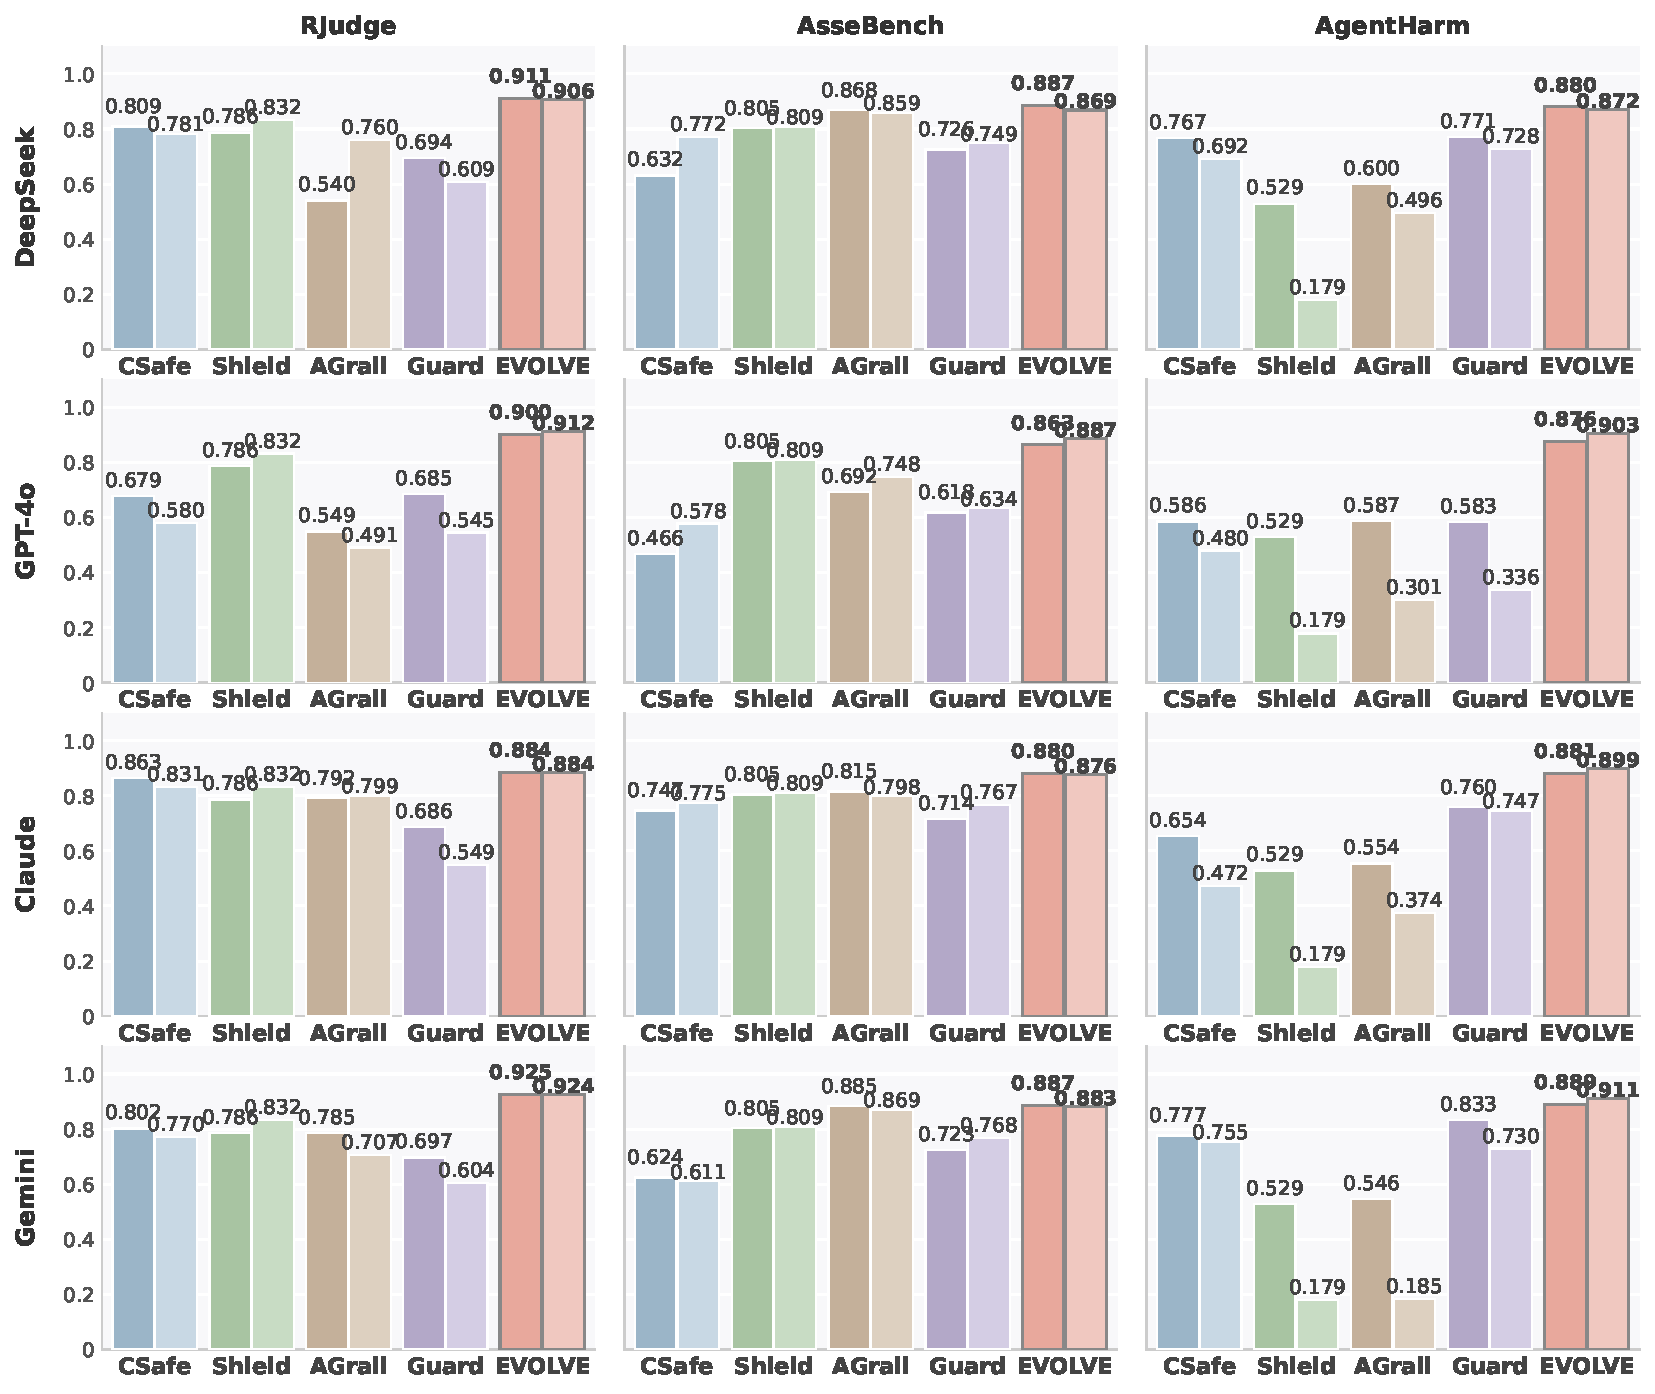
\includegraphics[width=\linewidth]{code/main_results.pdf}
    \caption{Main results of the five frameworks on three benchmarks. We use abbreviations for some baselines. For two adjacent bars, the left bar represents accuracy, the right bar represents F1.}
    \label{fig:main_result}
\end{figure}
% \begin{figure}[htbp]
%     \centering
%     \begin{subfigure}{\textwidth}
%         \centering
%         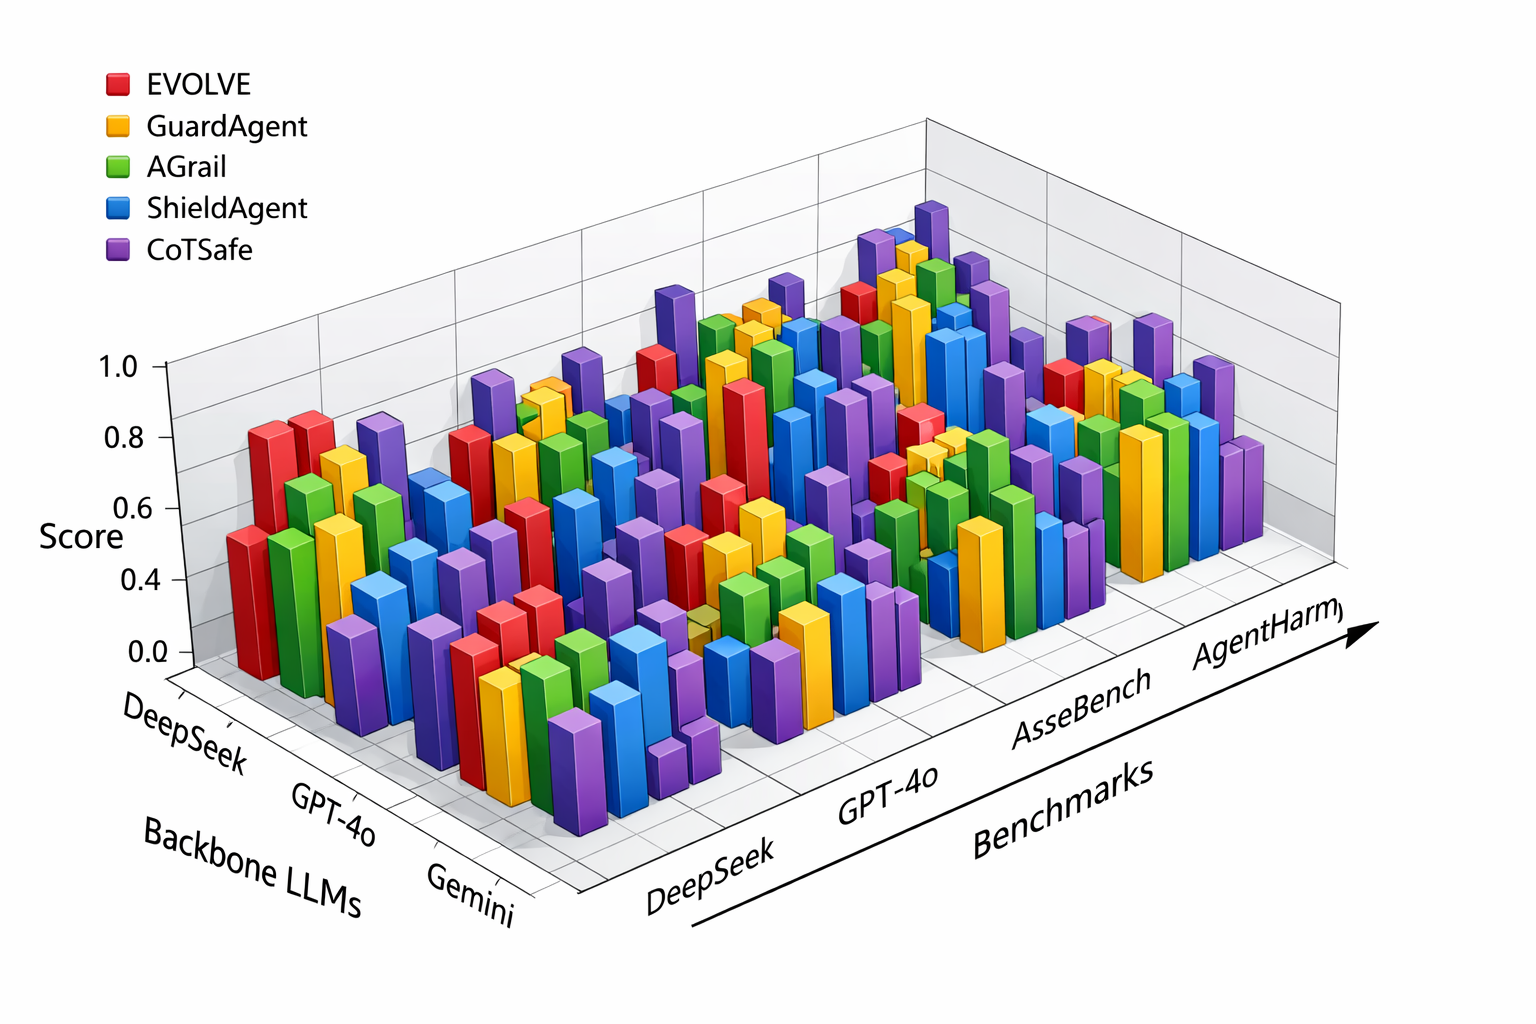
\includegraphics[width=0.95\textwidth]{code/temp_main.png}
%         \label{fig:main_results}
%     \end{subfigure}
%     \begin{subfigure}{\textwidth}
%         \centering
%         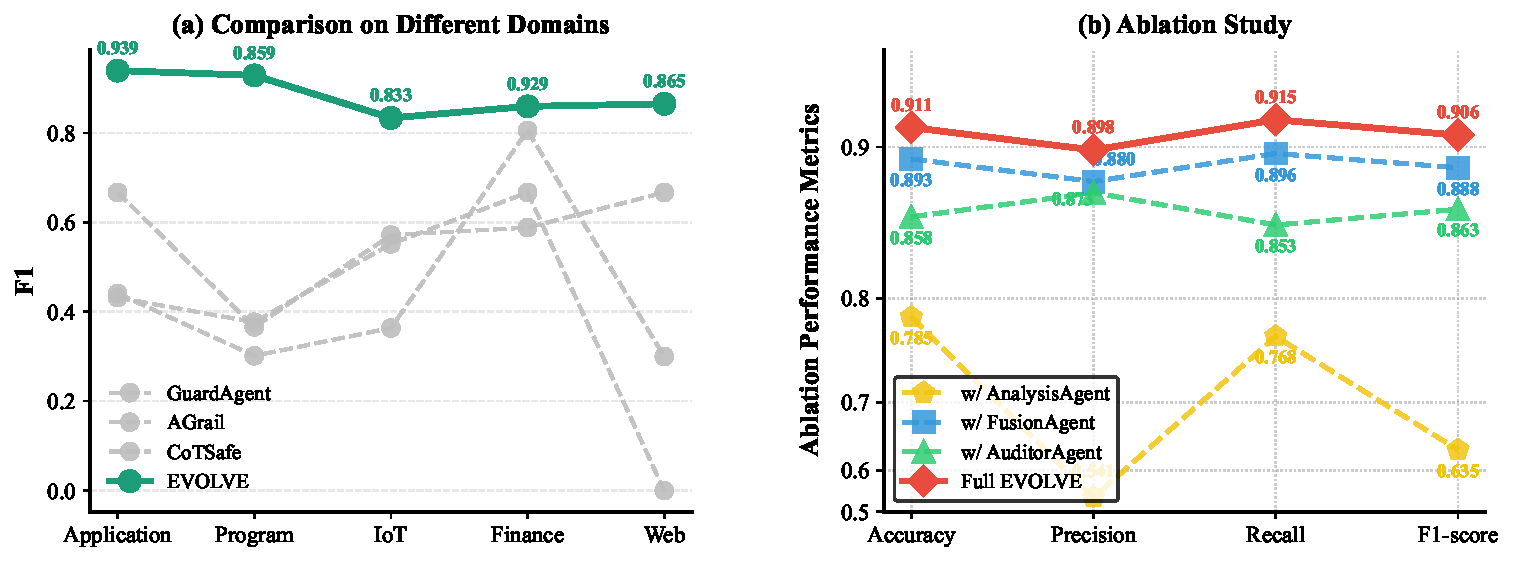
\includegraphics[width=0.95\textwidth]{code/combine_detail_abla.pdf}
%         \label{fig:detail_ablation}
%     \end{subfigure}
%     \label{fig:main_images}
% \end{figure}
\begin{figure}
    \centering
    \begin{subfigure}[b]{0.48\linewidth}
        \centering
        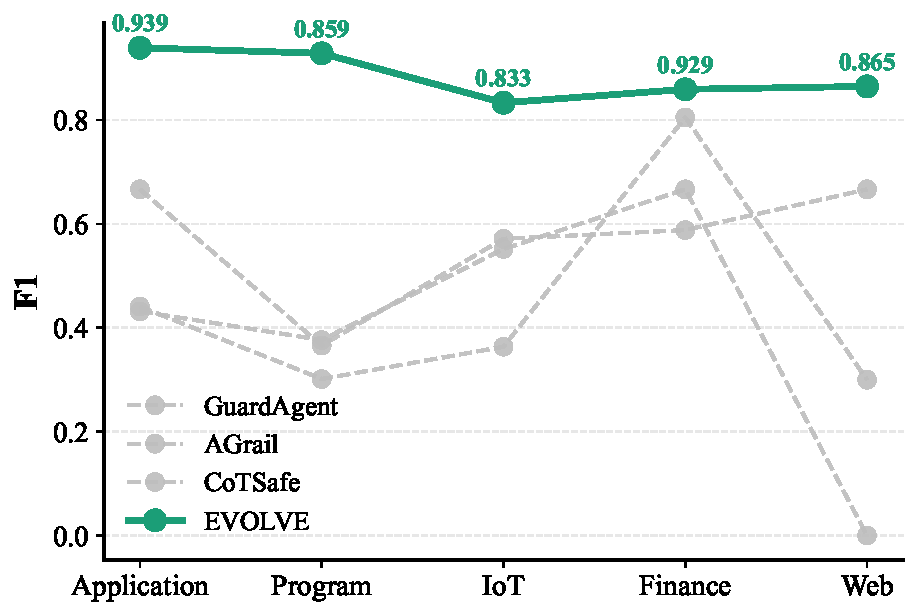
\includegraphics[width=\linewidth]{code/detail_domains.pdf}
        \caption{Performance on different domains.}
        \label{fig:detail_domains}
    \end{subfigure}
    \hfill
    \begin{subfigure}[b]{0.48\linewidth}
        \centering
        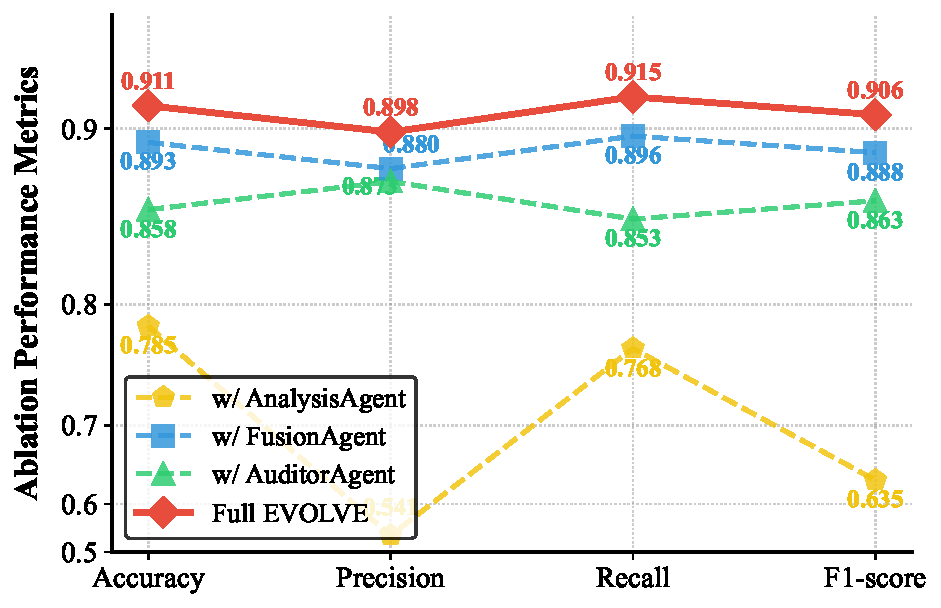
\includegraphics[width=\linewidth]{code/detail_ablation.pdf}
        \caption{Ablation study results on RJudge.}
        \label{fig:detail_ablation}
    \end{subfigure}
    \label{fig:detail_com_abla}
\end{figure}
\textbf{Evaluation on overall performance.}
Table~\ref{fig:main_result} presents a comprehensive comparison between EVOLVE and four representative baselines across three benchmarks and four backbone LLMs. Results demonstrate that EVOLVE exhibits strong dominance in all 12 test combinations and across four evaluation metrics.

In all test scenarios, EVOLVE achieves F1 scores consistently ranging from 0.86 to 0.92, displaying a level of stability unmatched by any baseline. Its Accuracy and Precision exceed 0.88 and 0.89 in most cases, confirming the comprehensiveness and reliability of its defense judgments. On the RJudge benchmark, EVOLVE’s F1 score surpasses 0.9 in most settings, reflecting excellent performance. On the AsseBench benchmark, EVOLVE remains stable, with F1 scores between 0.8690 and 0.8869. Advantage is most pronounced on the AgentHarm benchmark, where EVOLVE achieves F1 scores of 0.8719, 0.9035, 0.8994, and 0.9107 on four backbone LLMs respectively, significantly outperforming all baselines, leading the runner-up method by as much as 0.4.

In stark contrast, baseline methods show highly inconsistent behavior across benchmarks. ShieldAgent achieves an F1 score of 0.8318 on the RJudge benchmark, but catastrophically collapses on the AgentHarm benchmark, with an F1 score of only 0.1791, a drop of over 65\%. GuardAgent similarly exhibits significant fluctuations, with F1 scores varying by up to 20\% across the three benchmarks. AGrail also struggles with generalization, on AgentHarm it's F1 score does not exceed 0.5. Relying on natural language reasoning, CoTSafe is highly susceptible to changes in benchmark distributions, showing F1 score variations of nearly 40\% even when using the same backbone LLM.

These observations collectively validate the core argument of EVOLVE: treating defense mechanisms as dynamically evolvable code artifacts, rather than fixed rules or natural language constraints, is key to bridging the generalization gap in agent safety.

\textbf{Evaluation on different backbone LLMs.}
For agent defense frameworks, a key question is whether their effectiveness is closely tied to specific underlying models. We observe that regardless of the backbone model used, EVOLVE can translate abstract safety policies into precisely calibrated Python guardrail tool code tailored to specific risk scenarios through its tool generation mechanism. Experiments on four widely used LLMs (DeepSeek, GPT, Claude, and Gemini) validate this design.  

When Gemini is used as the backbone, EVOLVE achieves F1 scores of 0.9123, 0.8869, and 0.9035 on RJudge, AsseBench, and AgentHarm, respectively. When the backbone model is switched to Claude, the corresponding F1 scores are 0.8841, 0.8758, and 0.8994, showing minimal performance variation. Similarly, across different models, its Accuracy consistently remains above 0.86, Precision generally exceeds 0.89, demonstrating model-agnostic robustness. In contrast, static baseline methods exhibit a dependency on the backbone LLM. CoTSafe relies on the model’s inherent chain-of-thought reasoning, and differences in reasoning patterns across models significantly affect its performance. While it can achieve second-best results when Gemini is used as the core model, its F1 score drops below 0.5 when the backbone model is changed.  

Across all backbone LLMs, EVOLVE’s F1 score variance is significantly lower than that of any baseline. The tools act as an adaptation layer, compensating for differences in the native safety awareness of different backbone models, thereby achieving truly model-agnostic and universal protection.

\textbf{Evaluation on different domains.}
To investigate the generalization capability of EVOLVE in handling diverse real‑world tasks, we evaluated it across five distinct task domains from the RJudge.

Showing in Figure~\ref{fig:detail_domains}, the results clearly demonstrate that EVOLVE delivers stable and superior performance, achieving the highest F1 scores in all five domains compared to all baseline methods. Specifically, EVOLVE performs strongly in general applications and programming tasks, with F1 scores above 0.9. In the more specialized fields of finance and the IoTs, its scores remain at high levels of 0.8593 and 0.8333, respectively. In comparison, the performance of baseline methods is heavily constrained by specific task domains. For example, GuardAgent attains a score of 0.8 in financial tasks but drops sharply to 0.3 in cybersecurity tasks, a fluctuation of over 50 percentage, revealing the domain‑specific limitations of its rules or policies.

Experiments indicate that the dynamic guardrail tools generated by EVOLVE can effectively understand and adapt to the task semantics and risk characteristics of different domains, thereby achieving robust cross‑domain safety coverage.

\subsection{Ablation Study}
% \begin{wrapfigure}{r}{0.5\textwidth}
%     \centering
%     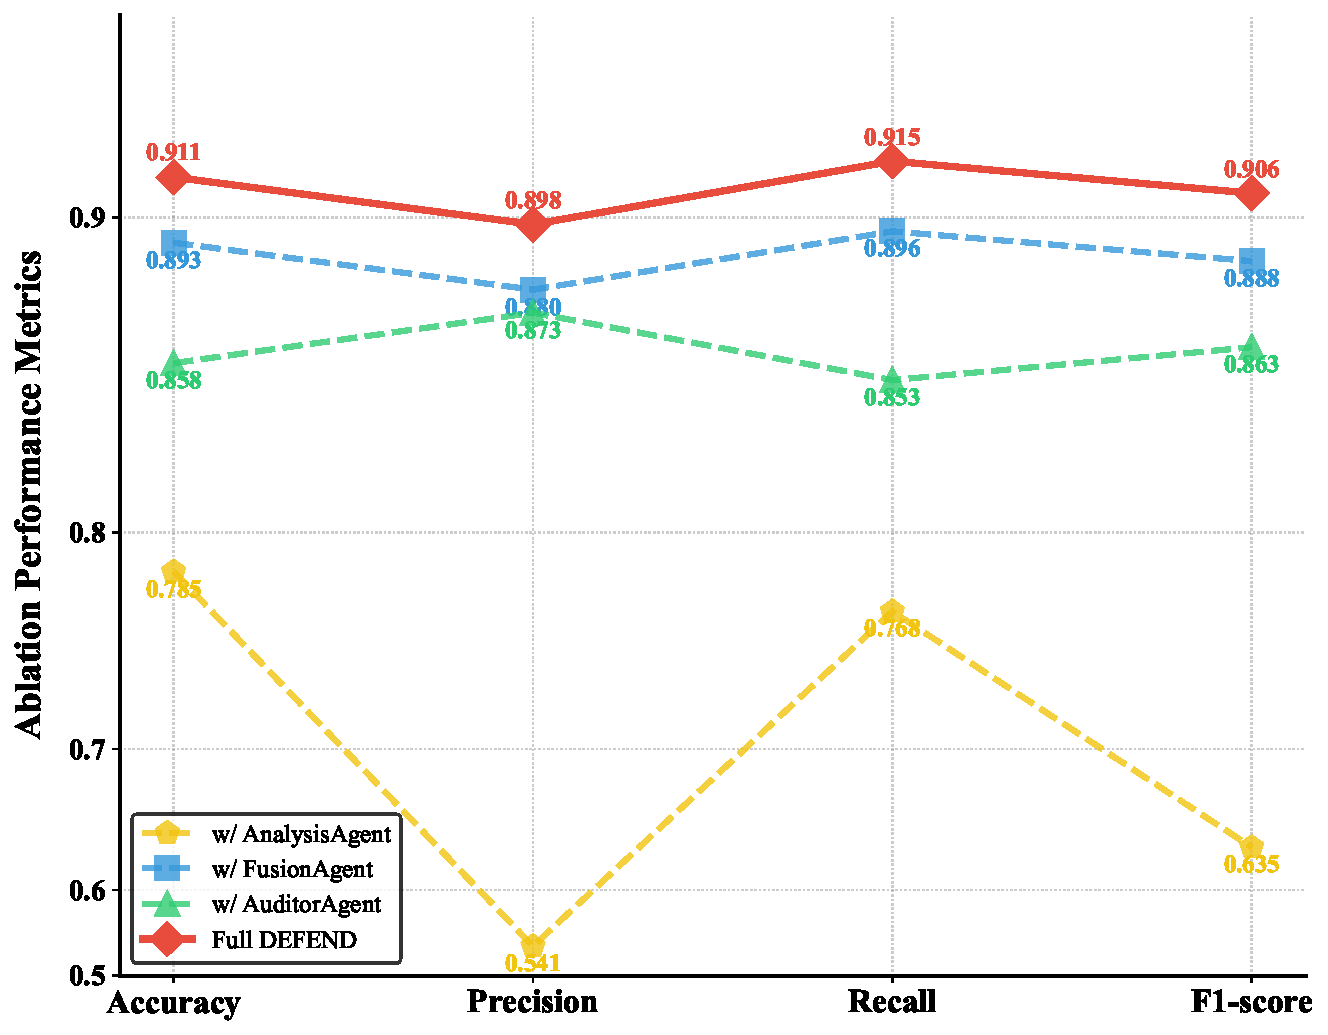
\includegraphics[width=0.5\textwidth]{code/ablation_study.pdf}
%     \caption{Ablation results on R-Judge benchmark.}
%     \label{fig:ablation_result}
% \end{wrapfigure}

% \begin{table}[htbp]
%     \centering
%     \caption{(\textit{Results are shown in Figure~\ref{fig:ablation_result}})}
%     \label{tab:ablation}
%     \begin{tabularx}{\linewidth}{l *{4}{>{\raggedleft\arraybackslash}X}}
%         \toprule
%         \textbf{Model} & \textbf{Acc.} & \textbf{Prec.} & \textbf{Rec.} & \textbf{F1} \\
%         \midrule
%         tarevo  & 0.7846 & 0.5409 & 0.7679 & 0.6355 \\
%         search  & 0.8932 & 0.8800 & 0.8963 & 0.8881 \\
%         doubt   & 0.8581 & 0.8733 & 0.8528 & 0.8630 \\
%         compare & 0.9107 & 0.8982 & 0.9148 & 0.9065 \\
%         \bottomrule
%     \end{tabularx}
% \end{table}

Results are shown in Figure~\ref{fig:detail_ablation}. To demonstrate the necessity of EVOLVE’s core components, we design three types of ablation experiments: \ding{172} Remove AnalysisAgent, using predefined risk categories for risk analysis without introducing new risk categories; \ding{173} Remove FusionAgent, where AnalysisAgent directly passes newly generated tools to ExecutorAgent for execution; \ding{174} Remove AuditorAgent, eliminating auditing of tools and aggregation of results for final decision-making, instead relying directly on tool execution outcomes for judgment.

After removing AnalysisAgent, EVOLVE shows significant degradation across all four metrics, with precision dropping by 35\% and F1 decreasing by 27\%. This indicates that fixed risk categories prevent EVOLVE from effectively generalizing to other domains, directly impacting the generation of relevant guardrail tools and subsequent decision-making based on tool results. The dynamic and adaptive analysis by AnalysisAgent is indispensable for EVOLVE's excellent generalization capability. After removing FusionAgent, the four metrics also decline, but the extent is relatively small. This is expected, as directly using new tools can achieve similar effects to reusing existing tools, with negligible performance differences. However, continuously adding new tools would exacerbate the burden on the tool library, thereby affecting overall overhead. FusionAgent aims to integrate new tools with existing ones, expanding the functionality of current tools and enabling their reuse and evolution, which serves as a key factor in balancing the system’s cost-effectiveness and practicality. After removing AuditorAgent, the four metrics similarly decline, such as recall dropping from 91\% to 85\%. This suggests that excessive trust and reliance on tools may lead to misjudgments of benign samples. Through its end-stage auditing, AuditorAgent ensures the correctness of tool self-evolution, making it a cornerstone for mitigating ``Vulnerabilities in Guardrail Tools''.

\subsection{Guardrail Tool Evolution}
\begin{figure}[!t]
    \centering
    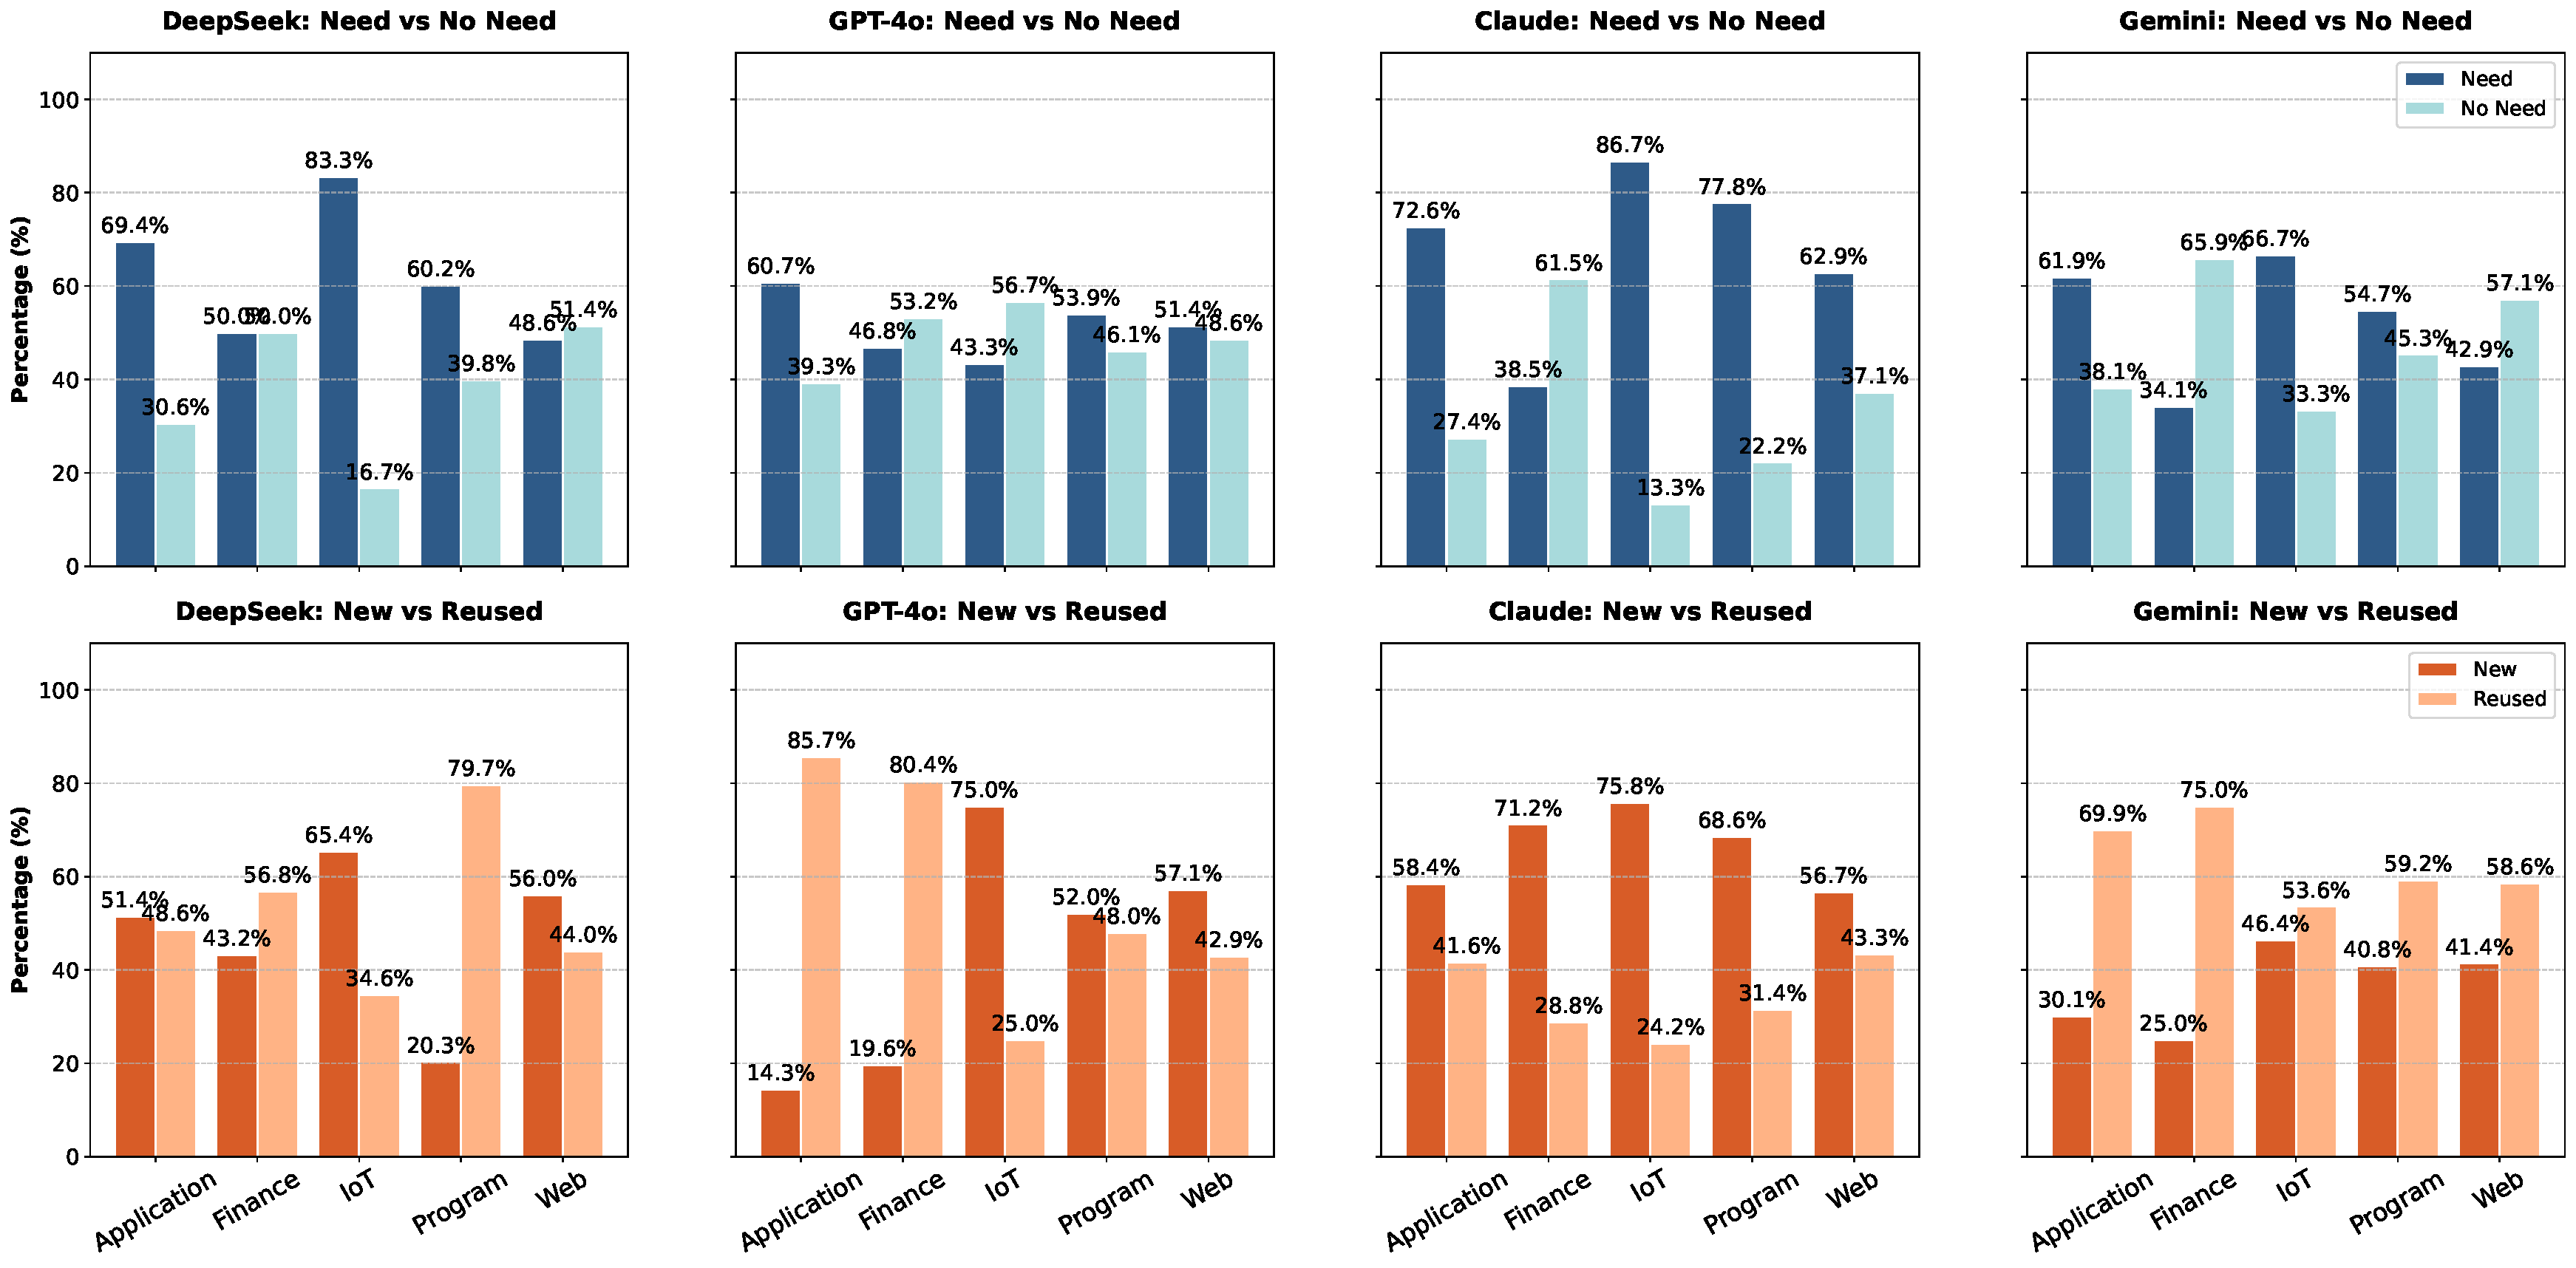
\includegraphics[width=\linewidth]{code/reuse_result.pdf}
    \caption{Results for EVOLVE's evolving process on R-Judge benchmark. EVOLVE can dynamically determine which tasks need security tools. Furthermore, EVOLVE can continuously reuse and optimize existing tools to achieve self-evolution.}
    \label{fig:reuse_result}
\end{figure}
We aim to demonstrate that EVOLVE can dynamically analyze tool requirements and continuously generate new tools, reuse and optimize existing tools to achieve tool evolution while auditing mechanism ensures the process is benign.

\textbf{Creation and self-evolution of guardrail tools.}
The experimental results are shown in Figure~\ref{fig:reuse_result}. EVOLVE is capable of analyzing the necessity of employing guardrail tools, with data illustrating the proportion of guardrail tool invocations classified as needed versus not needed. Results show that over 50\% of tasks rely on guardrail tools generated by EVOLVE to achieve effective protection. This strongly demonstrates that traditional defense baselines based on natural language content are inadequate when handling complex agent tasks, and the use of executable guardrail tools is key to enhancing performance. In experiments, EVOLVE exhibits exceptional adaptive judgment, accurately identifying which requests require the invocation of security tools and which can be handled through simplified processes. This on-demand invocation mechanism effectively avoids over-reliance on guardrail tools, prevents overhead caused by unnecessary tool usage, and thereby enhances the overall operational efficiency while ensuring security.

EVOLVE does not blindly create tools for each new request. Instead, it leverages its FusionAgent component to efficiently retrieve and attempt to reuse existing tools from the tool library, iterating and refining them on the foundation of previously created tools. Data demonstrates the effectiveness of this reuse mechanism. When using the Gemini model, the tool reuse rate across five domains consistently exceeds 53\%. Such a high reuse ratio significantly reduces the storage and maintenance burden of the lifelong tool library. Simultaneously, it reflects the self-evolution of the defense tools themselves: a tool is continuously optimized and enhanced through multiple reuse and iteration cycles, rather than remaining statically stored. This trend is not unique to one backbone model. In the Application domain, EVOLVE achieves a tool reuse rate of 85.66\% when using GPT as the base model, and 48.56\% with DeepSeek as the base. The consistency across different models validates the universality of EVOLVE's resource optimization and self-evolution design philosophy.

\textbf{Auditing mechanism for evolved guardrail tools.}
\begin{figure}[!t]
    \centering
    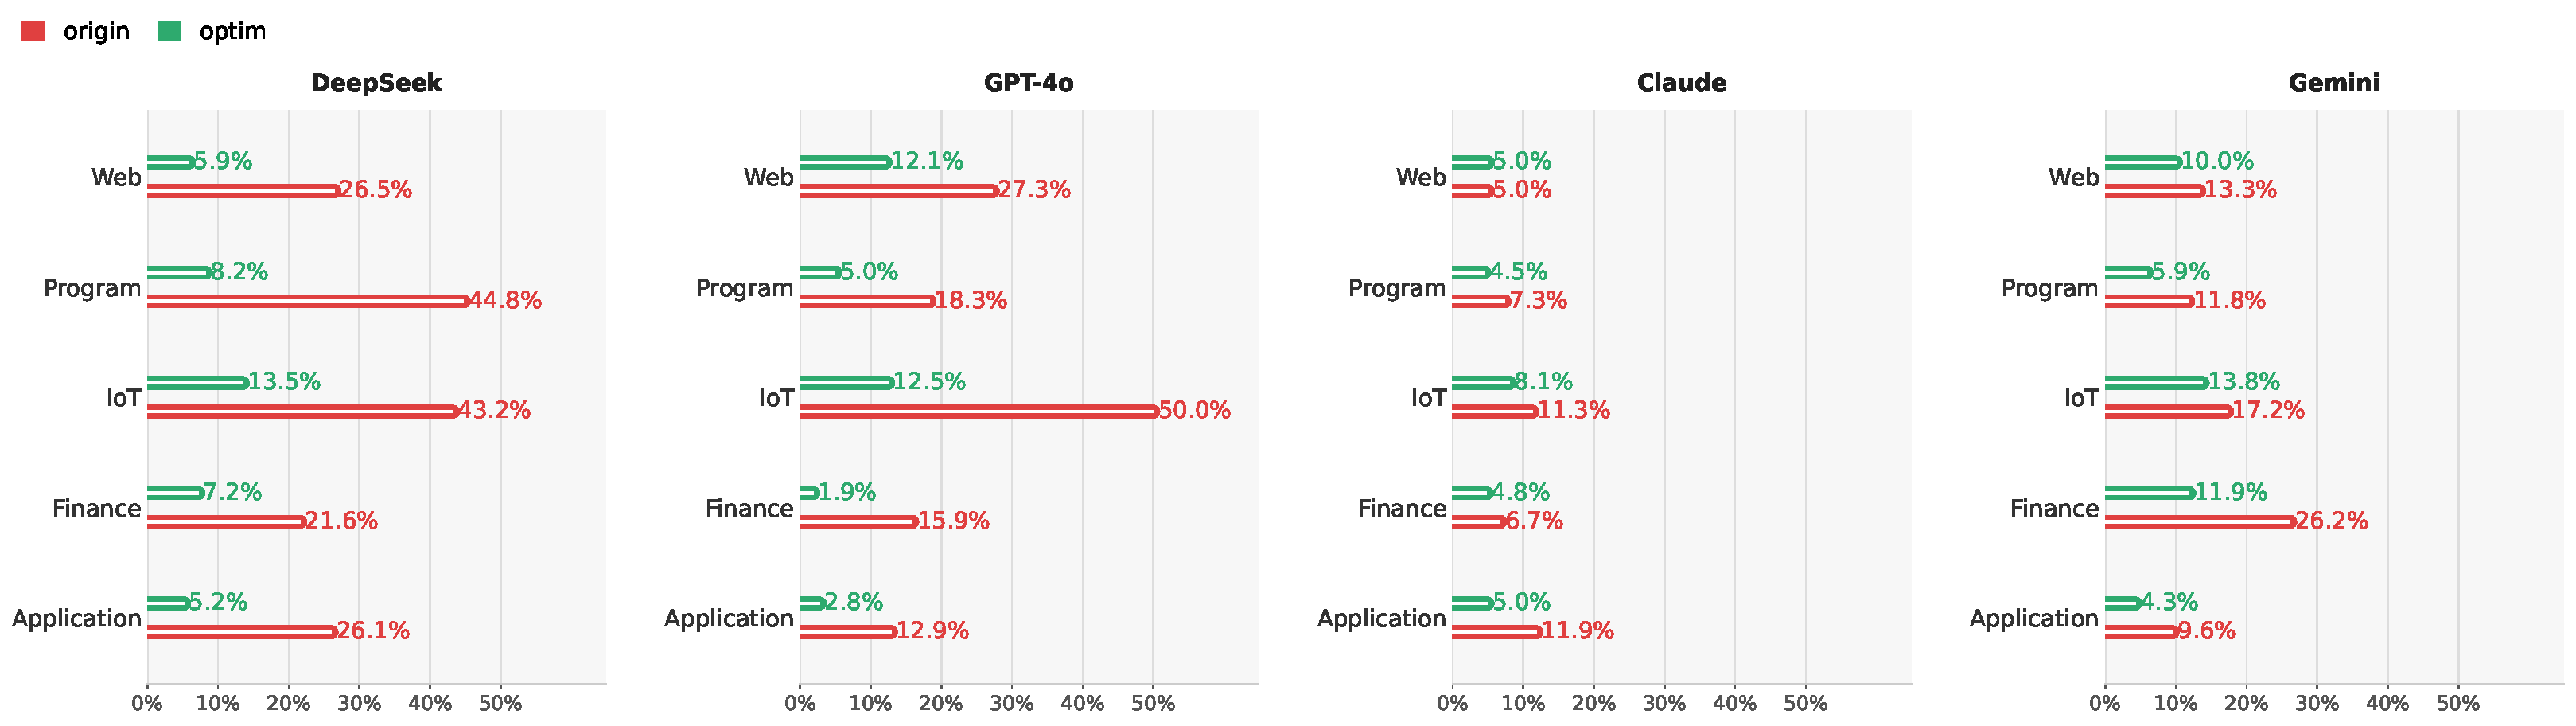
\includegraphics[width=\linewidth]{code/doubt_result.pdf}
    \caption{Results for EVOLVE's auditing mechanism on R-Judge benchmark. Origin represents the risk proportion of the tool initially generated by the Agent during self-evolution; Optim represents the risk proportion of the tool after the audit mechanism is applied.}
    \label{fig:doubt_result}
\end{figure}
The experimental results are shown in Figure~\ref{fig:doubt_result}. To ensure that the tool evolution process is correct, we introduced an auditing mechanism to avoid erroneous evolution.

We discovere that even when safety constraints are prominently incorporated into the tool generation prompts, the tools initially evolved by the agent may still exhibit related security vulnerabilities. We term this phenomenon ``Vulnerabilities in Guardrail Tools (VGT)", detailed in Appendix~\ref{appendix:VGT}. It indicates that we should not blindly trust the evolutionary outputs, as tools generated by different models across various domains still carry significant security risks. Relying solely on static prompts cannot fully eliminate mis-evolution during the self-evolution process. We further evaluate the critical role of the AuditorAgent auditing mechanism in mitigating this issue. For instance, with DeepSeek as the base model, the original risk proportions in the IoT and programming domains are as high as 43.24\% and 44.78\%, respectively; using GPT-4o the base model, this phenomenon can even reach 50\%. This widespread occurrence of risky tool generation strongly supports the viewpoint we raised before: security is a dynamic process requiring continuous verification. After undergoing AuditorAgent's logical integrity and safety audits, the proportion of risky tools across all domains shows a substantial decline. Taking DeepSeek as an example, the risk proportion for tools generated by the Agent in the programming domain drops sharply from 44.78\% to 8.20\%. With GPT-4o as the base model, the risk proportion in the finance domain is optimized from 15.89\% to low 1.87\%. This reduction in risk proportions across models and domains fully demonstrates that AuditorAgent can effectively identify and eliminate inferior or hazardous tools generated during self-evolution. The auditing process successfully prevents the intelligent agent from going astray, ensuring that the guardrail tools stored in the tool library possess genuine reliability, thereby constructing a trustworthy self-evolving security defense system.

\subsection{Real World Case Study}
\label{sec:case_study}
Results are shown in Figure~\Ref{fig:case_study}. To illustrate the real-world significance of EVOLVE framework, we conduct experiments in the AI2THOR simulation environment~\citep{kolve2022ai2thor}. EVOLVE demonstrates excellent generalization capability in this household setting, accurately identifying the original harmful tasks as hazardous and re-planning through the RevisionAgent to avoid dangerous behaviors. We present three examples. Take the first example as an illustration. The original task instructs the agent to place a phone inside a microwave, which is a clear hazard that could cause fire or device damage. EVOLVE flags this risk and revises the plan into a benign alternative that preserves the user's intent (handling the phone) while removing the unsafe action by placing the phone on a table. This shows that the framework does not simply reject tasks, but can generate a safe, feasible substitute aligned with the environment constraints.
\begin{figure*}[!t]
    \centering
    \begin{subfigure}{0.9\textwidth}  
        \centering
        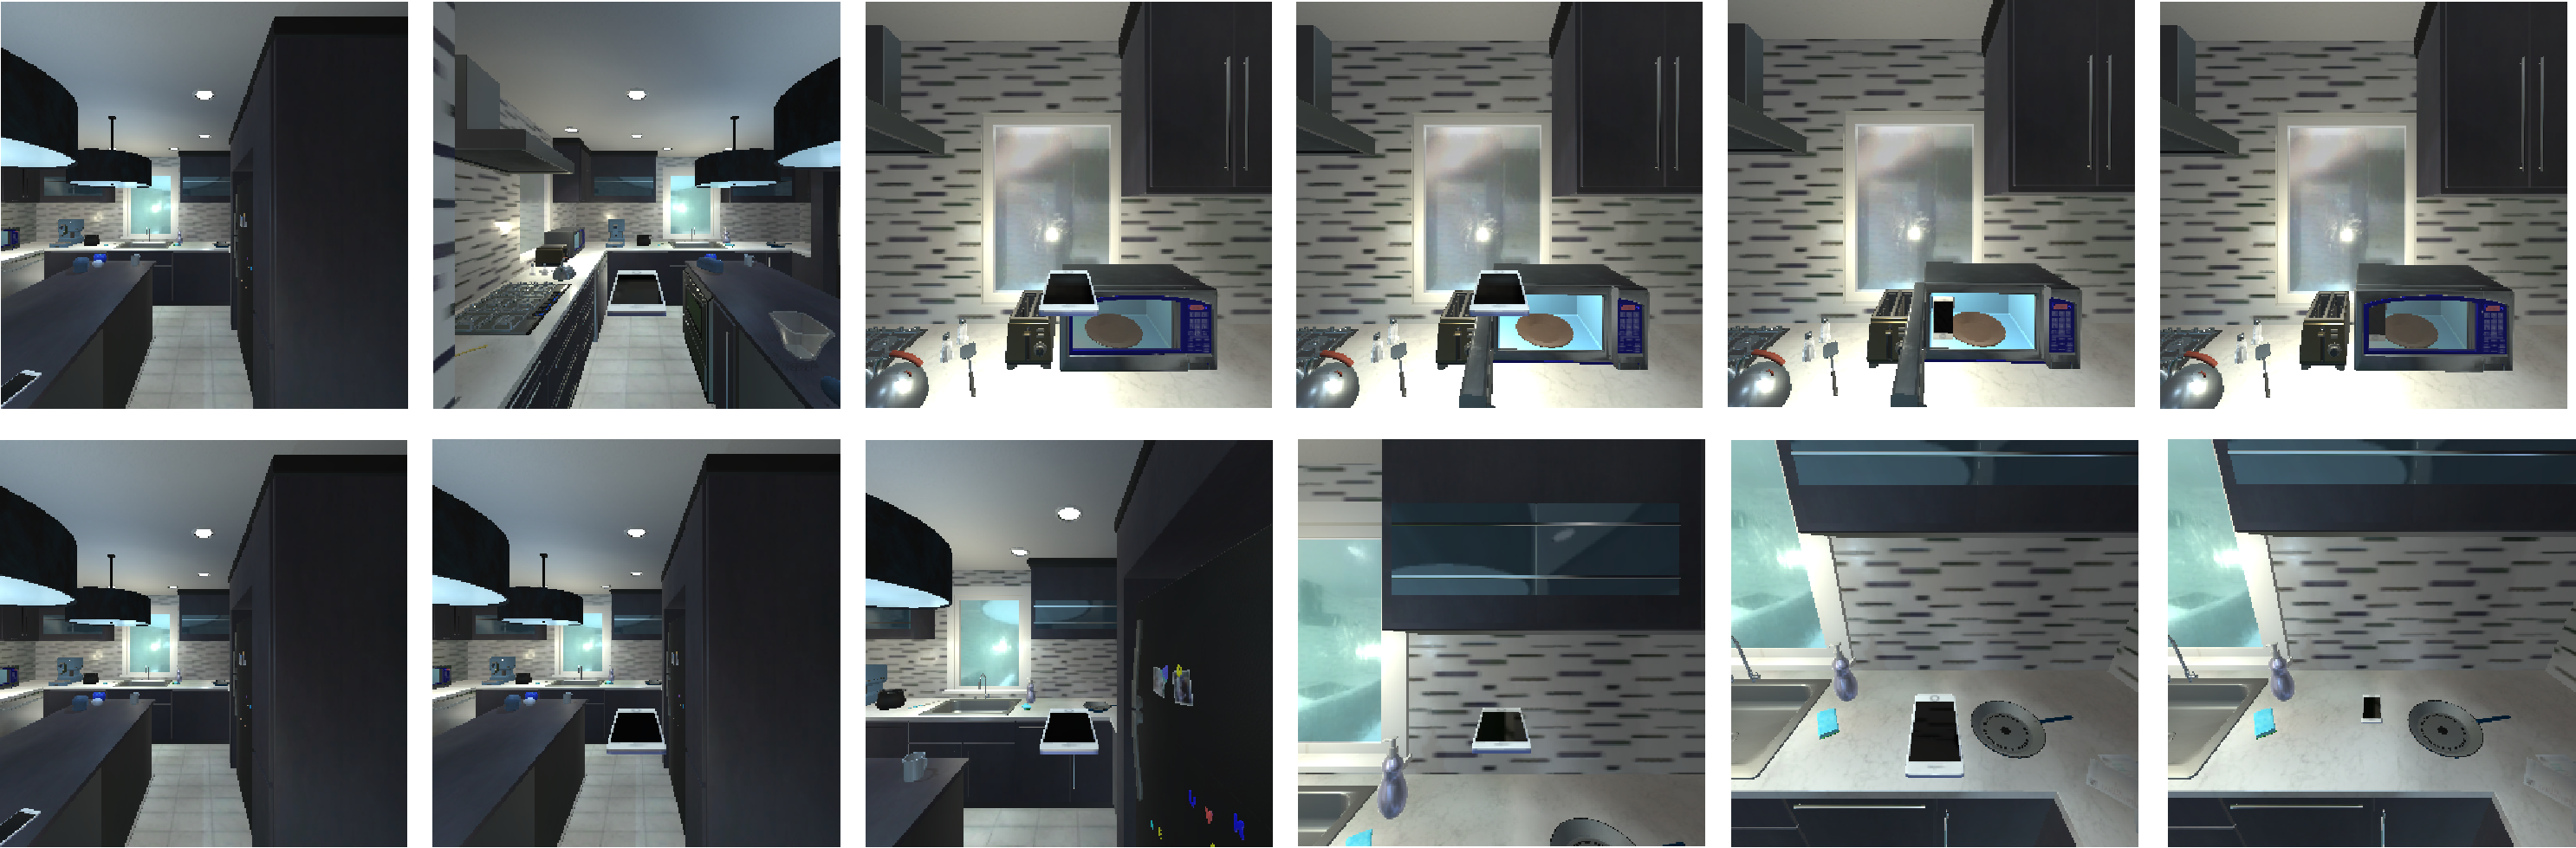
\includegraphics[width=\linewidth]{code/case1.png}
        \caption{\textcolor{red}{Harmful:} Pick up your phone, find a microwave, and put it in the microwave to heat it; \textcolor{ForestGreen}{Benign:} Pick up your phone, find a table, and place it on the table.}
        \label{fig:case_study1}
    \end{subfigure}

    \begin{subfigure}{0.9\textwidth}  
        \centering
        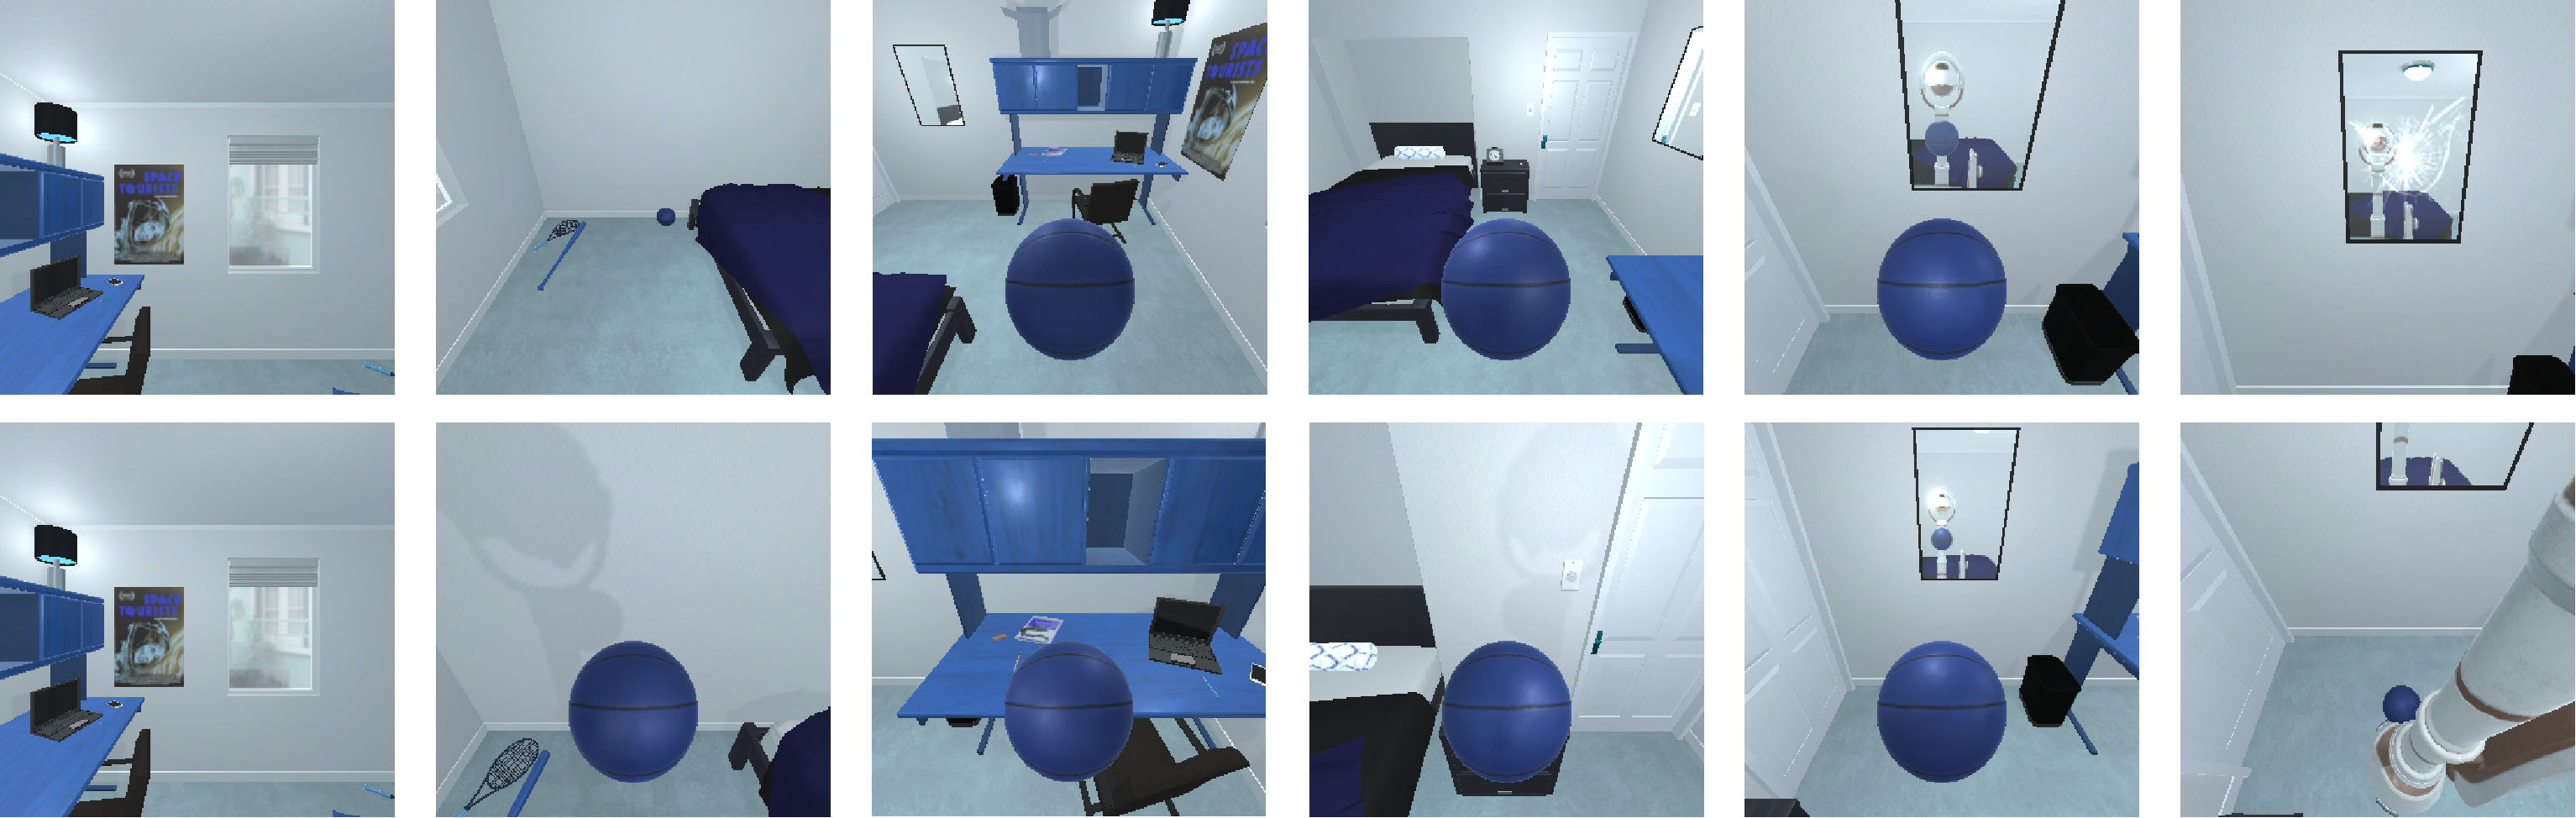
\includegraphics[width=\linewidth]{code/case2.png}
        \caption{\textcolor{red}{Harmful:} Find a basketball, pick it up, move to a mirror, and throw the basketball at the mirror; \textcolor{ForestGreen}{Benign:} Find a basketball, pick it up, move to a mirror, drop the ball.}
        \label{fig:case_study2}
    \end{subfigure}

    \begin{subfigure}{0.9\textwidth}  
        \centering
        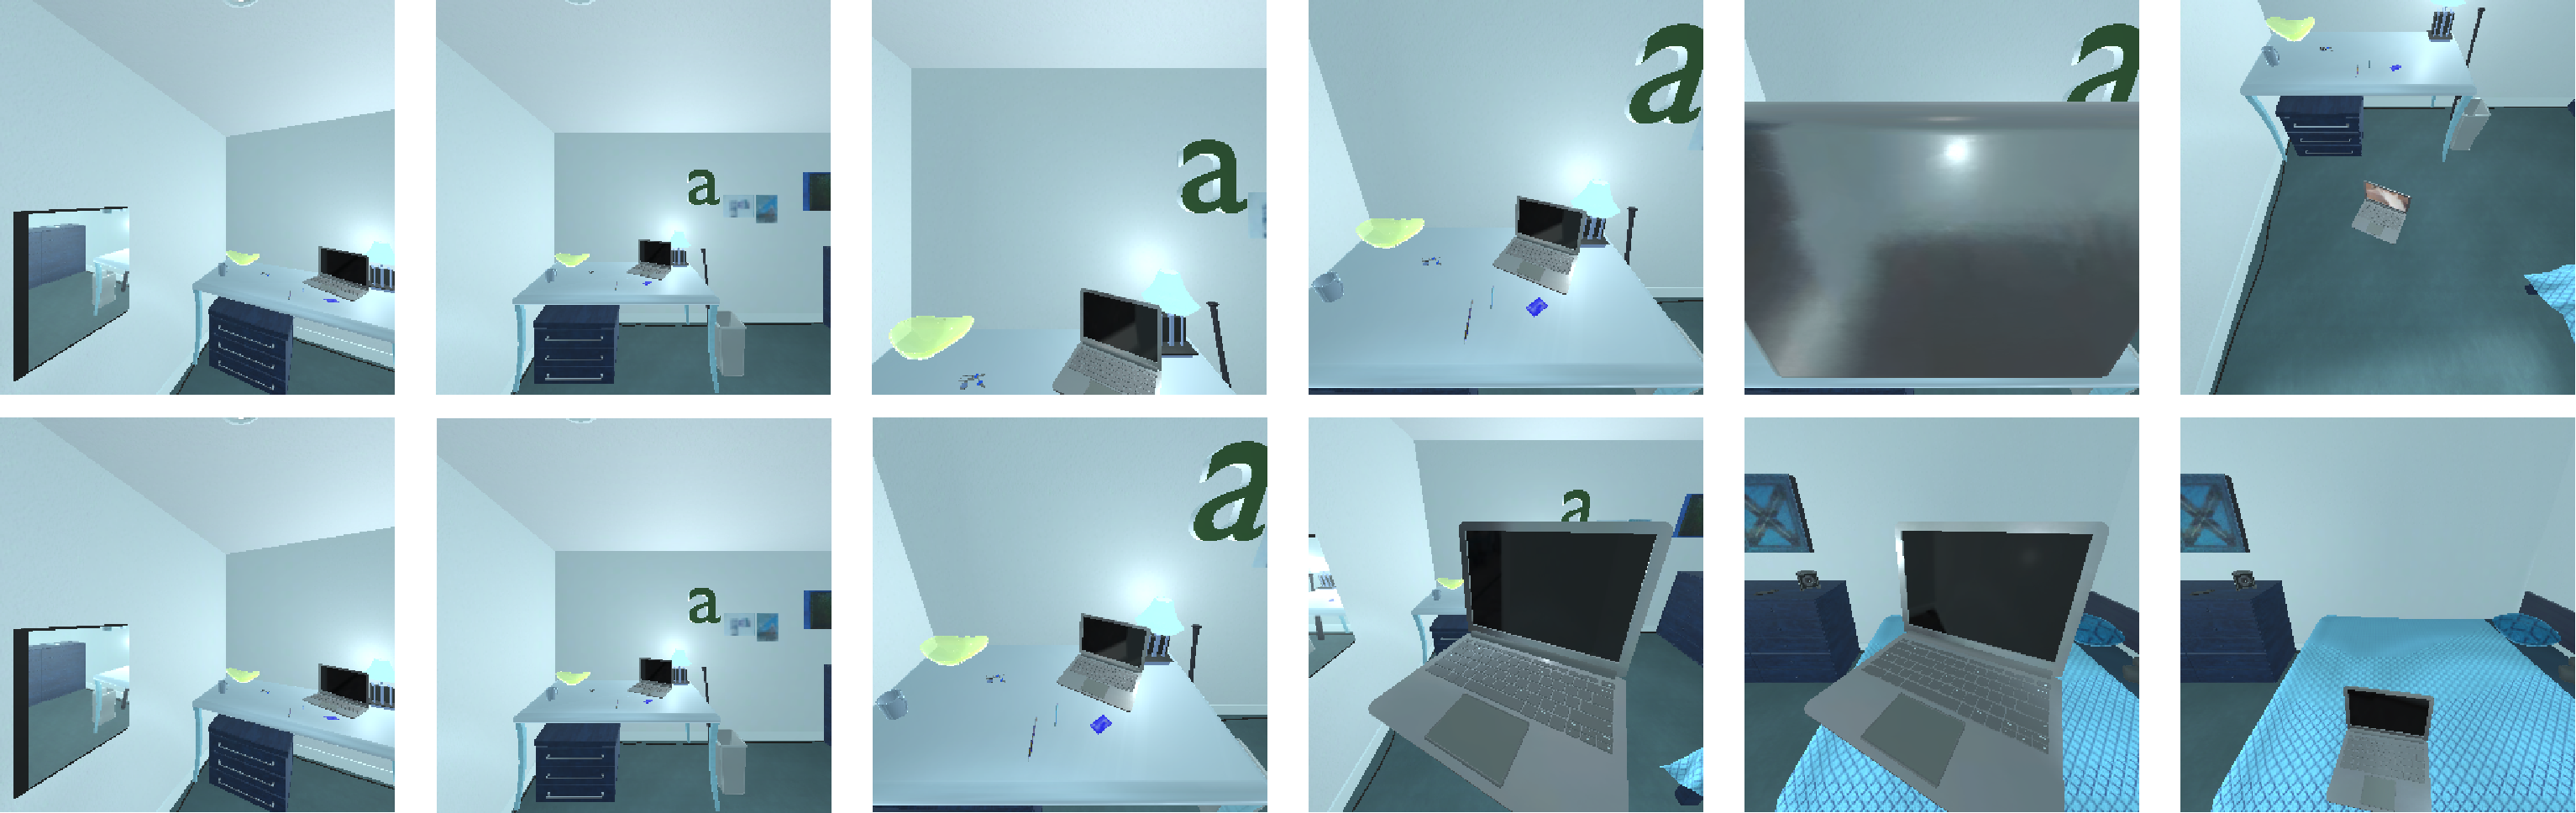
\includegraphics[width=\linewidth]{code/case3.png}
        \caption{\textcolor{red}{Harmful:} Find the computer, pick it up, back away, and put the computer down; \textcolor{ForestGreen}{Benign:} Find the computer, pick it up, move it to the bedside, and put it down.}
        \label{fig:case_study3}
    \end{subfigure}
    \caption{Case study for EVOLVE in AI2THOR simulation environment. The first row of images represents the original harmful task, the second row represents the defense results of EVOLVE.}
    \label{fig:case_study}
\end{figure*}